
\chapter{\label{sec:app:charmless}Charmless background}

\minitoc


Figures \ref{allchamrmless0Run1} and \ref{allchamrmless5Run1} show the fits to data in the D mass sidebands after a \Dz FD significance cut of zero and 5 respectively for Run 1 data. Figures \ref{allchamrmless0Run2} and \ref{allchamrmless5Run2} show the equivalent plots for Run 2 data. Plots show that the charmless contribution is reduced to a negligible level in all modes except for \decay{\Dz}{\pip\pim} where there may still be a residual contribution. 

\begin{figure}[h]
\centering
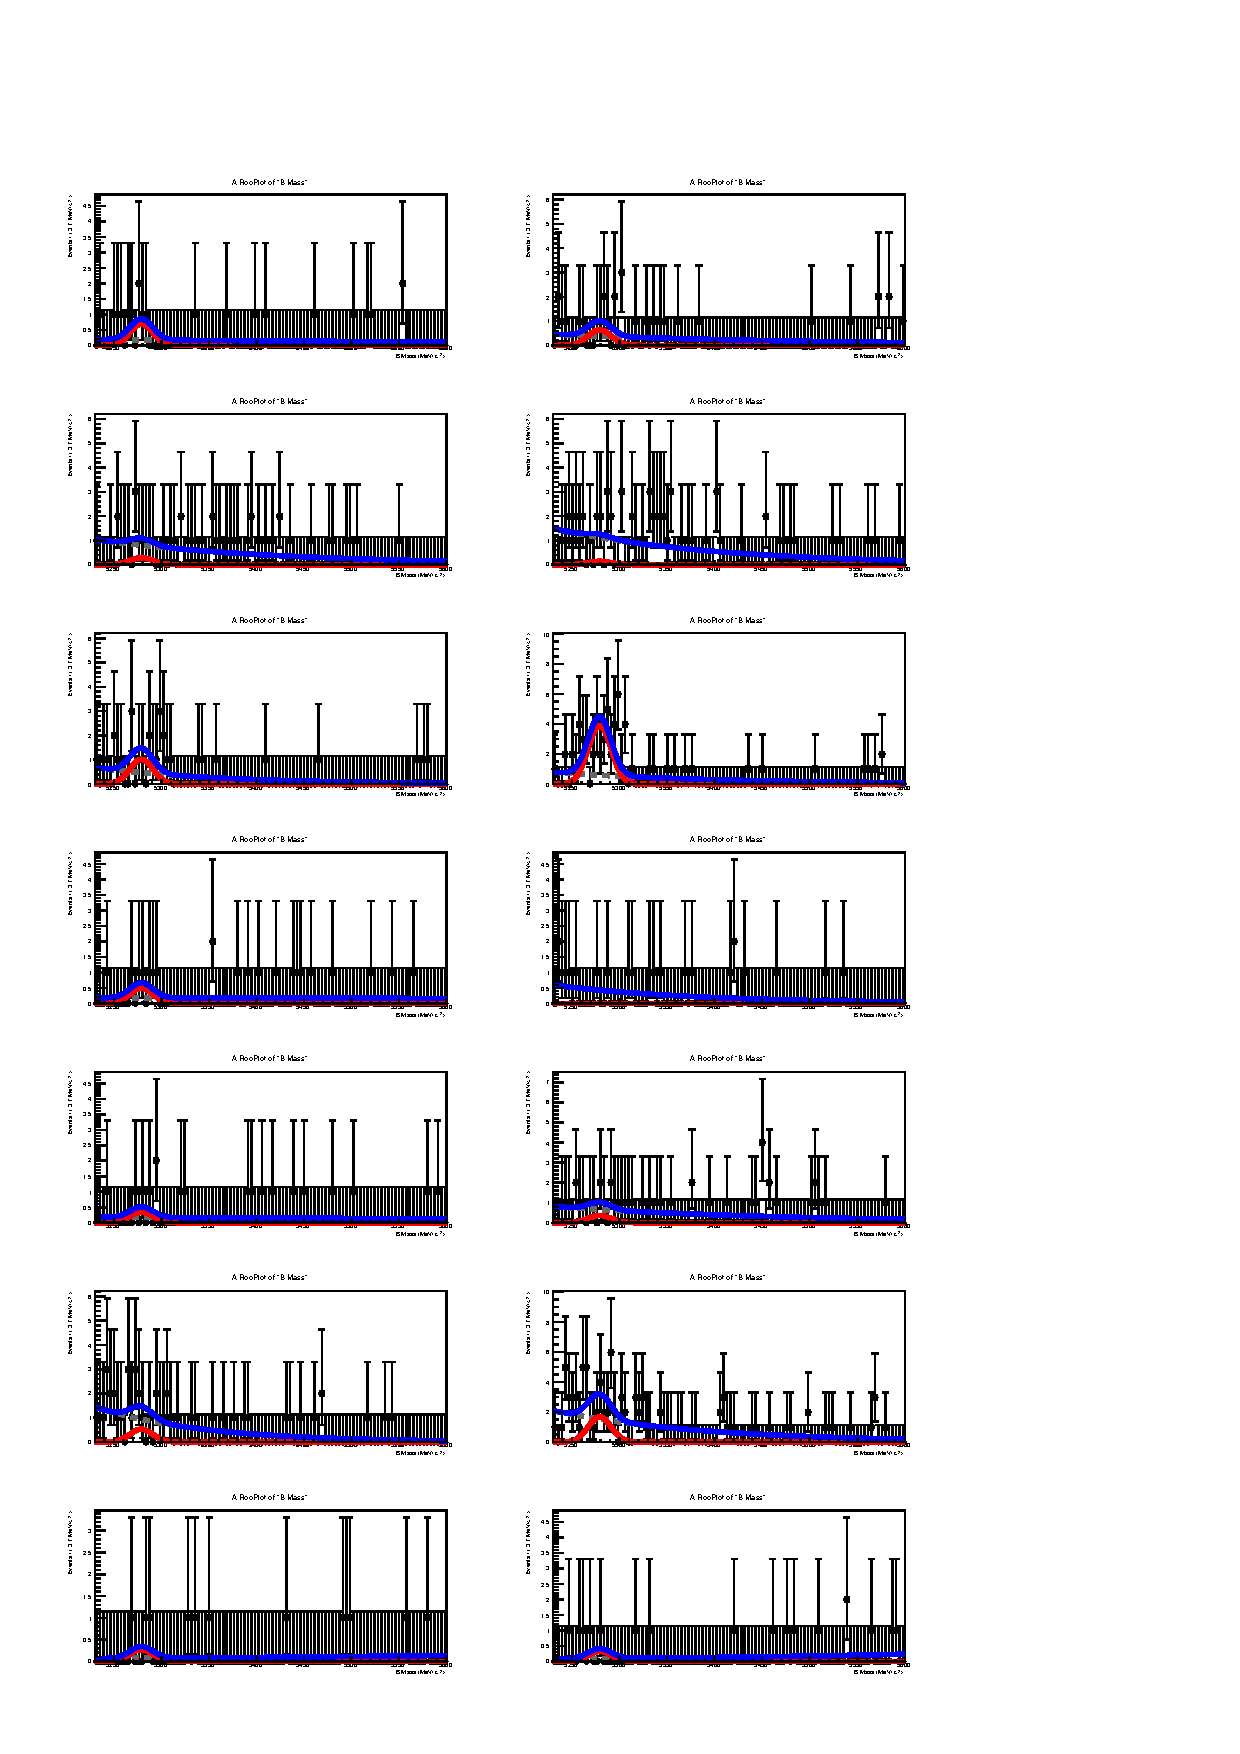
\includegraphics[width=0.65\linewidth]{figures/backgrounds/charmlessFits_FD0_run1.pdf}
\put(-250,470) {(a)}
\put(-100,470) {(b)}
\put(-250,400) {(c)}
\put(-100,400) {(d)}
\put(-250,330) {(e)}
\put(-100,330) {(f)}
\put(-250,260) {(g)}
\put(-100,260) {(h)}
\put(-250,190) {(i)}
\put(-100,190) {(j)}
\put(-250,120) {(k)}
\put(-100,120) {(l)}
\put(-250,40) {(m)}
\put(-100,40) {(n)}
\caption{Fits to be refitted B mass taking candidates from the D mass sidebands after a FD significance cut of zero for (a) $K\pi$ LL, (b) $K\pi$ DD, (c) $KK$ LL, (d) $KK$ DD, (e) $\pi\pi$ LL, (f) $\pi\pi$ DD, (g) $\pi K$ LL, (h) $\pi K$ DD, (i) $K\pi\pi\pi$ LL, (j) $K\pi\pi\pi$ DD, (k) $\pi\pi\pi\pi$ LL, (l) $\pi\pi\pi\pi$ DD, (m) $\pi K\pi\pi$ LL, and (n) $\pi K\pi\pi$ DD.. A Gaussian is used to model the signal and an exponential for the combinatoric background}
\label{allchamrmless0Run1}
\end{figure}

\begin{figure}[h]
\centering
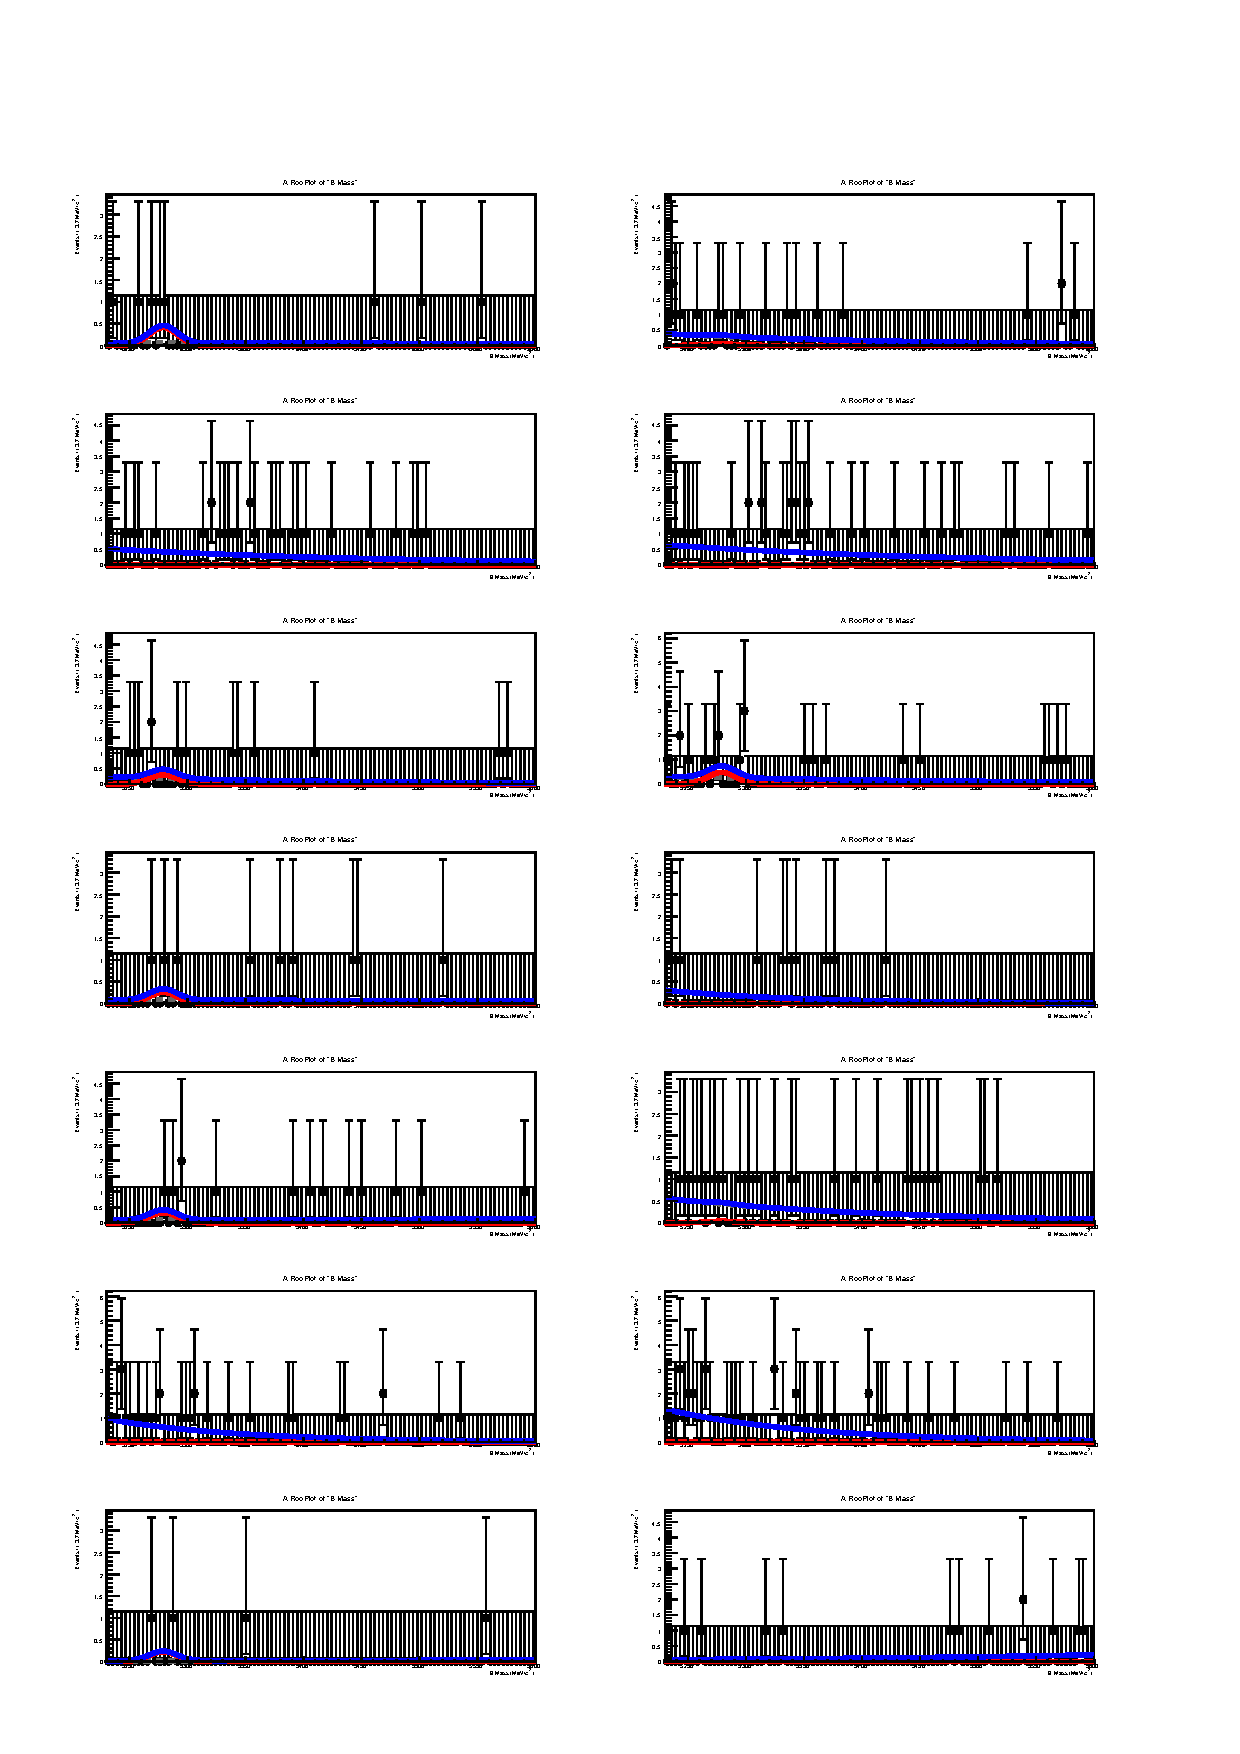
\includegraphics[width=0.8\linewidth]{figures/backgrounds/charmlessFits_FD2_run1.pdf}
\put(-250,470) {(a)}
\put(-100,470) {(b)}
\put(-250,400) {(c)}
\put(-100,400) {(d)}
\put(-250,330) {(e)}
\put(-100,330) {(f)}
\put(-250,260) {(g)}
\put(-100,260) {(h)}
\put(-250,190) {(i)}
\put(-100,190) {(j)}
\put(-250,120) {(k)}
\put(-100,120) {(l)}
\put(-250,40) {(m)}
\put(-100,40) {(n)}
\caption{Fits to be refitted B mass taking candidates from the D mass sidebands after a FD significance cut of 2$\sigma$ for (a) $K\pi$ LL, (b) $K\pi$ DD, (c) $KK$ LL, (d) $KK$ DD, (e) $\pi\pi$ LL, (f) $\pi\pi$ DD, (g) $\pi K$ LL, (h) $\pi K$ DD, (i) $K\pi\pi\pi$ LL, (j) $K\pi\pi\pi$ DD, (k) $\pi\pi\pi\pi$ LL, (l) $\pi\pi\pi\pi$ DD, (m) $\pi K\pi\pi$ LL, and (n) $\pi K\pi\pi$ DD.. A Gaussian is used to model the signal and an exponential for the combinatoric background}
\label{allchamrmless5Run1}
\end{figure}

\begin{figure}[h]
\centering
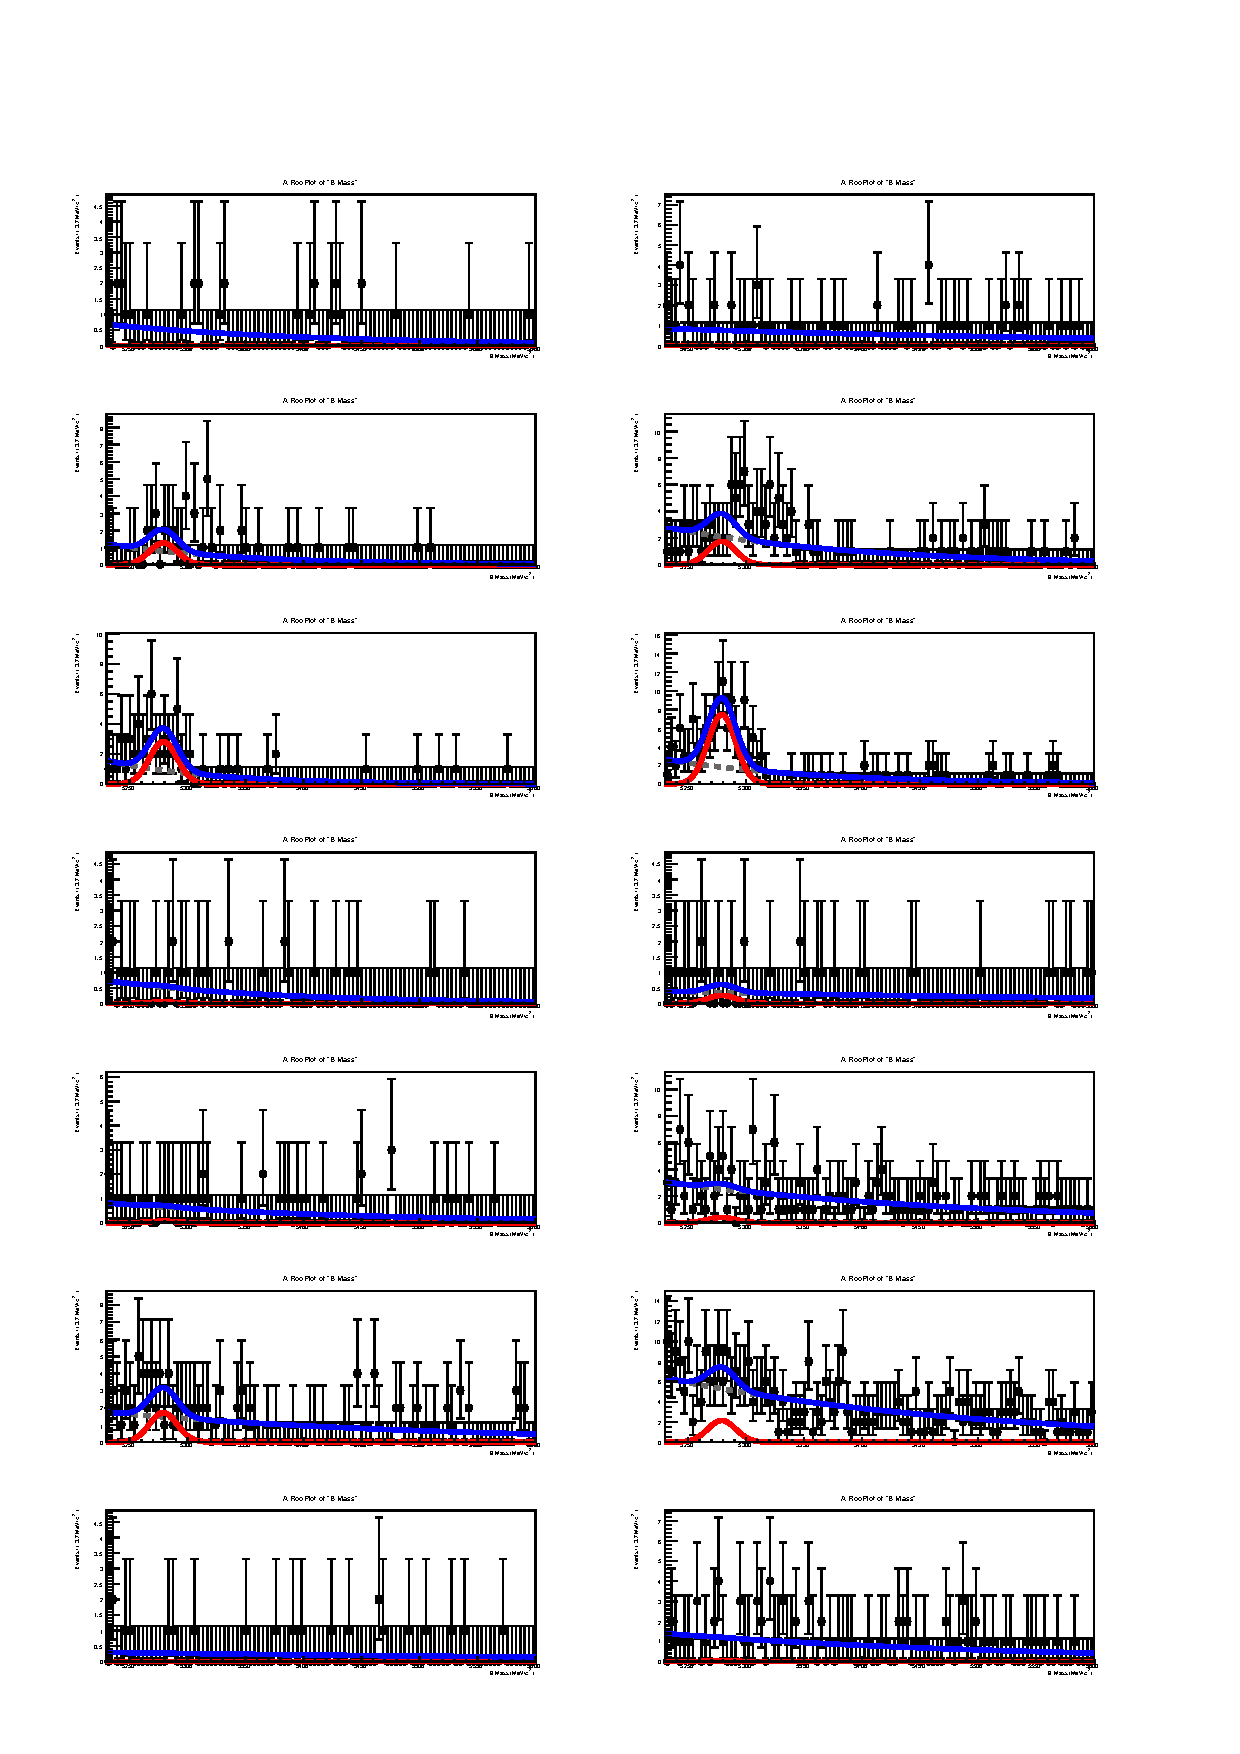
\includegraphics[width=0.8\linewidth]{figures/backgrounds/charmlessFits_FD0_run2.pdf}
\put(-250,470) {(a)}
\put(-100,470) {(b)}
\put(-250,400) {(c)}
\put(-100,400) {(d)}
\put(-250,330) {(e)}
\put(-100,330) {(f)}
\put(-250,260) {(g)}
\put(-100,260) {(h)}
\put(-250,190) {(i)}
\put(-100,190) {(j)}
\put(-250,120) {(k)}
\put(-100,120) {(l)}
\put(-250,40) {(m)}
\put(-100,40) {(n)}
\caption{Fits to be refitted B mass taking candidates from the D mass sidebands after a FD significance cut of zero for (a) $K\pi$ LL, (b) $K\pi$ DD, (c) $KK$ LL, (d) $KK$ DD, (e) $\pi\pi$ LL, (f) $\pi\pi$ DD, (g) $\pi K$ LL, (h) $\pi K$ DD, (i) $K\pi\pi\pi$ LL, (j) $K\pi\pi\pi$ DD, (k) $\pi\pi\pi\pi$ LL, (l) $\pi\pi\pi\pi$ DD, (m) $\pi K\pi\pi$ LL, and (n) $\pi K\pi\pi$ DD.. A Gaussian is used to model the signal and an exponential for the combinatoric background}
\label{allchamrmless0Run2}
\end{figure}

\begin{figure}[h]
\centering
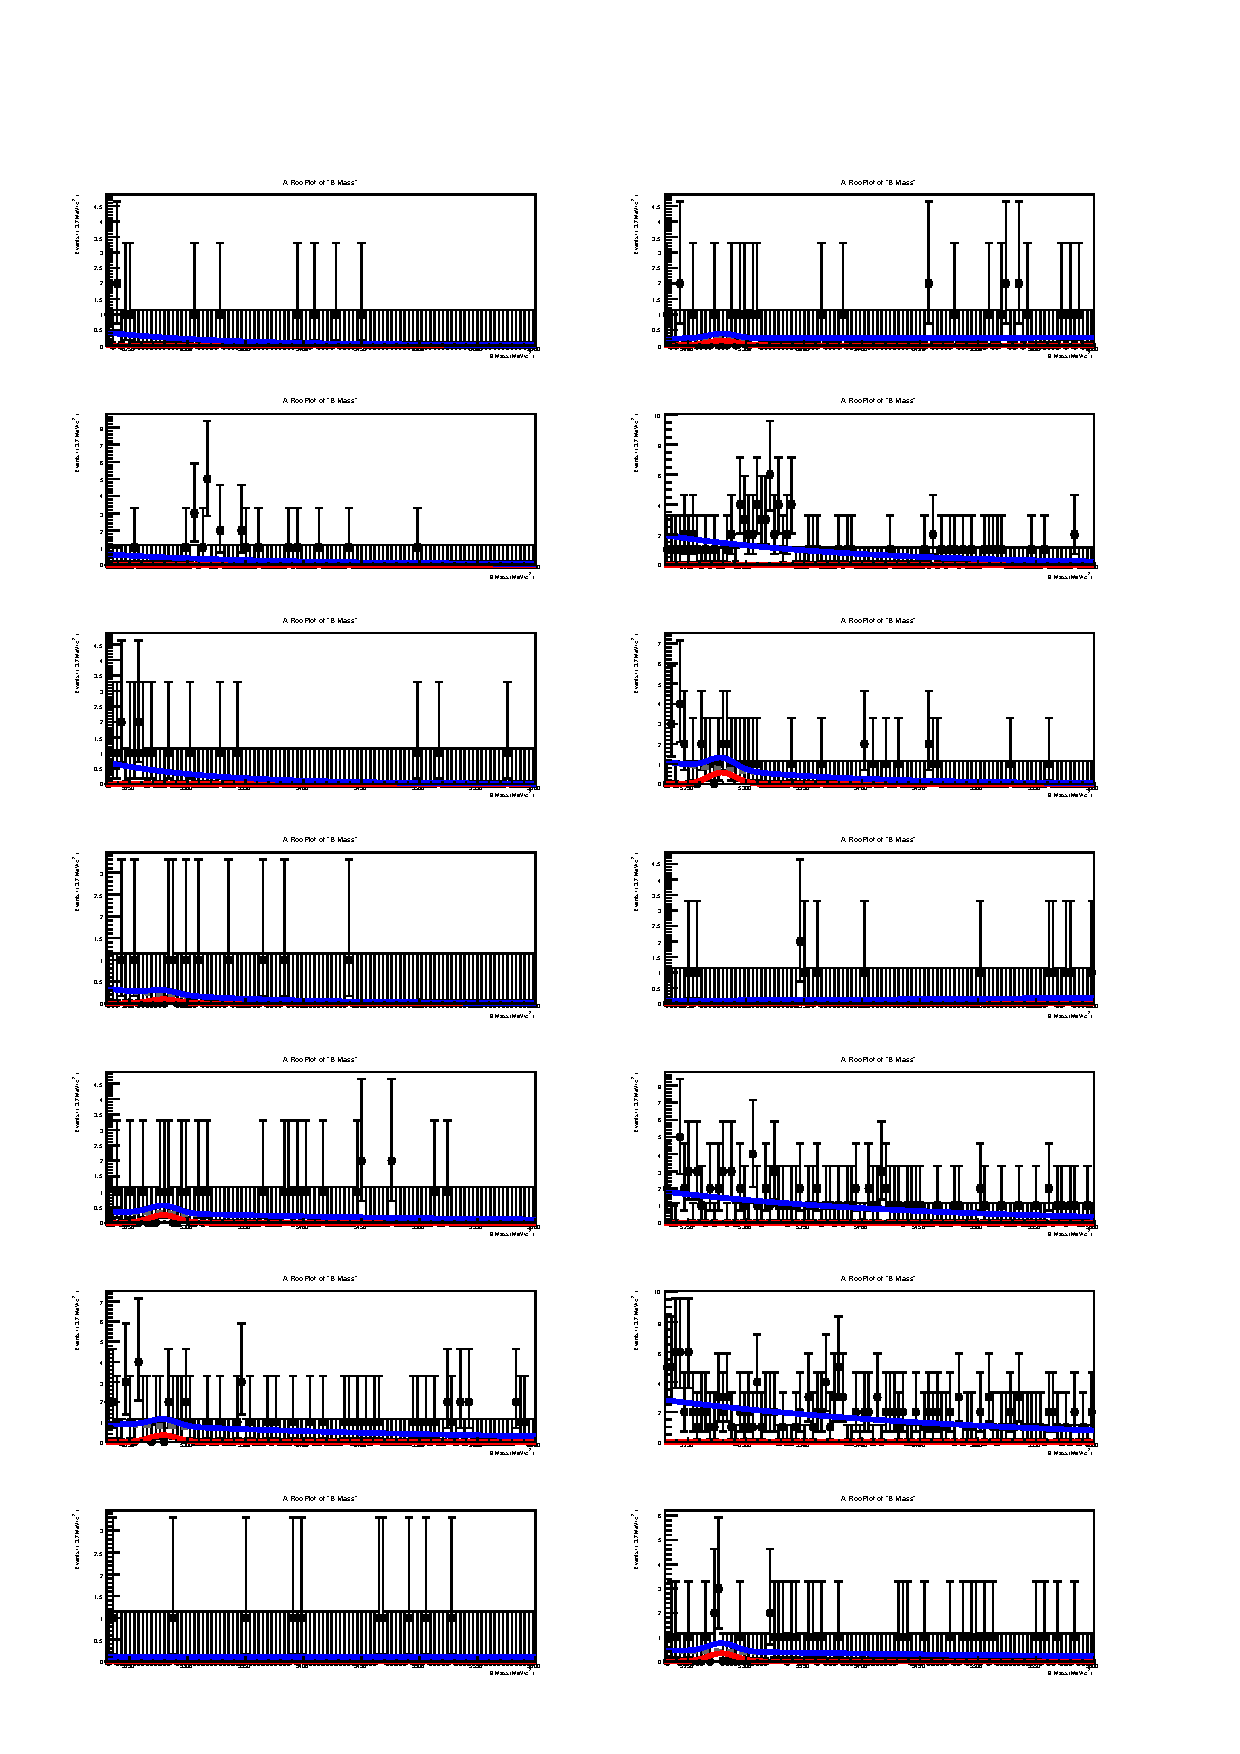
\includegraphics[width=0.8\linewidth]{figures/backgrounds/charmlessFits_FD2_run2.pdf}
\put(-250,470) {(a)}
\put(-100,470) {(b)}
\put(-250,400) {(c)}
\put(-100,400) {(d)}
\put(-250,330) {(e)}
\put(-100,330) {(f)}
\put(-250,260) {(g)}
\put(-100,260) {(h)}
\put(-250,190) {(i)}
\put(-100,190) {(j)}
\put(-250,120) {(k)}
\put(-100,120) {(l)}
\put(-250,40) {(m)}
\put(-100,40) {(n)}
\caption{Fits to be refitted B mass taking candidates from the D mass sidebands after a FD significance cut of 2$\sigma$ for (a) $K\pi$ LL, (b) $K\pi$ DD, (c) $KK$ LL, (d) $KK$ DD, (e) $\pi\pi$ LL, (f) $\pi\pi$ DD, (g) $\pi K$ LL, (h) $\pi K$ DD, (i) $K\pi\pi\pi$ LL, (j) $K\pi\pi\pi$ DD, (k) $\pi\pi\pi\pi$ LL, (l) $\pi\pi\pi\pi$ DD, (m) $\pi K\pi\pi$ LL, and (n) $\pi K\pi\pi$ DD. A Gaussian is used to model the signal and an exponential for the combinatoric background}
\label{allchamrmless5Run2}
\end{figure}

\clearpage